%%%%%%%%%%%%%%%%%%%%%%%%%%%%%%%%%%%%%%%%%
% Beamer Presentation
% LaTeX Template

\documentclass{beamer}
\mode<presentation> {
\usetheme{Warsaw}
}

\usepackage{multicol}
\usepackage[russian]{babel}
\usepackage{graphicx} 
\usepackage{hyperref}

\title[Introduction to Python]{Function, Module and Class} 
\author{Sugarkhuu Radnaa} 
\institute[]
{
Py4Econ in Ulaanbaatar \\ 
\medskip
\textit{py4econ@gmail.com} 
}
\date{}  % 

\begin{document}

\begin{frame}
\titlepage % Print the title page as the first slide
\end{frame}

\begin{frame}
    \frametitle{Week 6: Learning objectives}
    Get to know: 
    \begin{enumerate}
        \item Functions and Modules
        \item Class (OOP basics)         
    \end{enumerate}
\end{frame}


%------------------------------------------------
\section{Function} 
%------------------------------------------------

\begin{frame}
    \frametitle{Function}
    Function - not to repeat one action again and again
        \begin{center}
            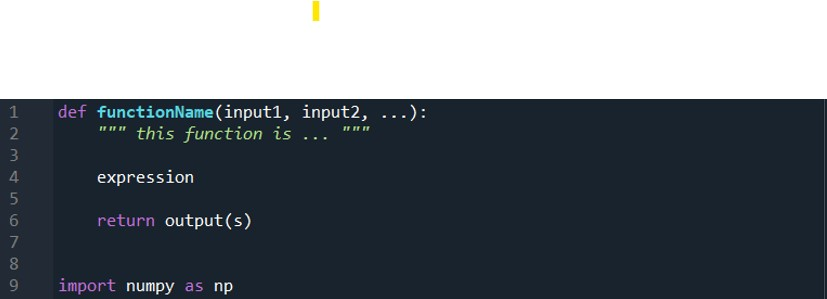
\includegraphics[scale=0.5]{figures/function.jpg}
        \end{center}        
    \end{frame}
    
    \begin{frame}
    \frametitle{Documenting a function is crucial!}
    Docstring prototype
            \begin{center}
                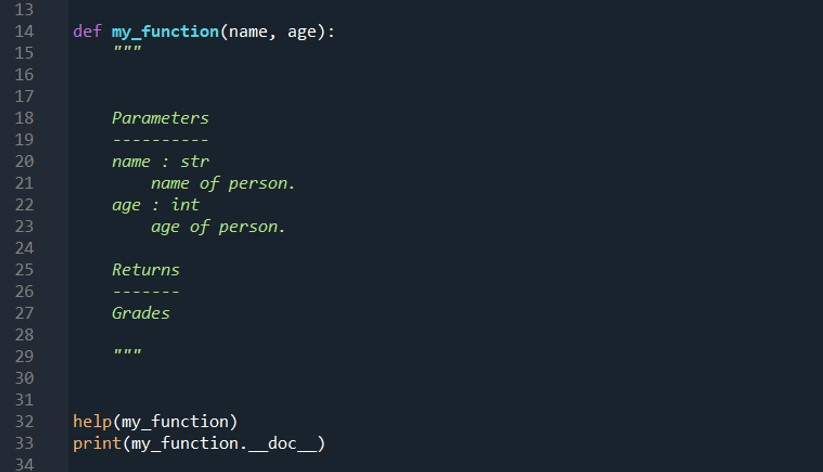
\includegraphics[scale=0.5]{figures/documentation.jpg}
            \end{center}
    \end{frame}
    
    \begin{frame}
    \frametitle{Function arguments}
        \begin{itemize}
            \item Positional (“input”) 
            \item Keyword (“input=value”) - with a default value
            \item Optional positional (*args)
            \item Optional keyword (**kwargs)        
        \end{itemize}
    \end{frame}
    
    
    \begin{frame}
    \frametitle{Scope of variable}
        \centering
        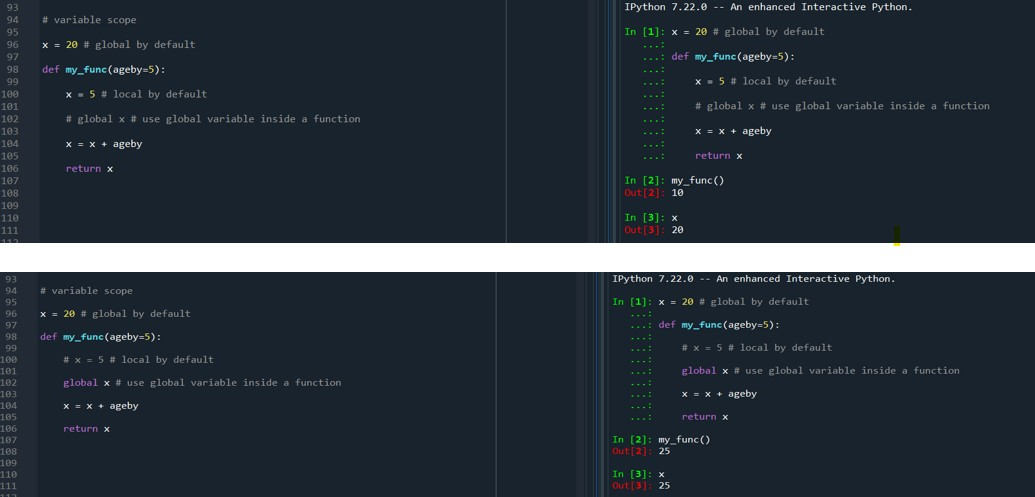
\includegraphics[scale=0.5]{figures/variable_scope.jpg}
    \end{frame}
    
%------------------------------------------------
\section{Module} 
%------------------------------------------------

    \begin{frame}
    \frametitle{Module}
    
    As your program gets longer, you may want
    \begin{itemize}
        \item to split it into several files 
        for easier maintenance
        \item to use also a handy function that
        you have written in several programs without copying its definition into each 
        program.
    \end{itemize}
    
    \vskip 2mm 
    
    To support this, Python has a way to put definitions in a file
    and use them. Such a file is called a \textit{module}; definitions from 
    a module can be imported into other modules or script. 
    
    \end{frame}
    
    
    \begin{frame}
    \frametitle{Class – OOP philosophy}
    
    \textbf{Def:} Object-oriented programming (OOP) is a computer programming 
    model that organizes software design around data, or objects, 
    rather than functions and logic. An object can be defined as a 
    data field that has unique attributes and behavior.
    \vskip 2mm 
    Important concepts:
        \begin{itemize}
            \item Object (instance)
            \item Method
            \item Inheritance (super, child classes)
            \item Setters and getters
            \item Variable accessibility – Public/Private/Protected
        \end{itemize}
    \end{frame}

    \begin{frame}
        \frametitle{Additional reading: Why is “class” useful?}
        Please read most upvoted answer by "dantiston":
         \url{https://stackoverflow.com/questions/33072570/when-should-i-be-using-classes-in-python} 
    \end{frame}

    
%------------------------------------------------
\section{Homework} 
%------------------------------------------------

\begin{frame}
    \frametitle{Homework}
    \begin{enumerate}
        \item Task 1
        \item Task 2
        \item Task 3
    \end{enumerate}

    \vskip 2mm
    \begin{itemize}
        \item Submit your result as a Github repository
        \item Deadline: 1 week %15 January, 2022
    \end{itemize}

\end{frame}


\begin{frame}
    \frametitle{Task 1: Function arguments}
    Jupyter notebook дээр зөвхөн args, зөвхөн args=value, зөвхөн *args, 
    зөвхөн **kwargs аргументуудтай (4 тусдаа функц) болон эдгээрийн холимог 
    (2 функц) байгуулж, ажиллуулж үзүүл. Нийт 6 функц.
\end{frame}

\begin{frame}
    \frametitle{Task 2: Class}
    Create a bank deposit class which you can 
    \begin{itemize}
        \item withdraw money
        \item deposit 
        \item check the balance
    \end{itemize}
    Show on Jupyter notebook how it works
\vskip 2mm
Examples: 
\tiny
    \begin{itemize}
        \item \url{https://www.engineeringbigdata.com/python-atm-code-for-account-balance-withdraw-and-deposit-functions/}
        \item \url{https://www.geeksforgeeks.org/python-program-to-create-bankaccount-class-with-deposit-withdraw-function/}
        \item \url{https://www.vtupulse.com/python-programs/python-program-using-classes-and-objects-to-deposit-and-withdraw-money-in-a-bank-account/}
        \item Tkinter GUI - \url{https://www.youtube.com/watch?v=SF-enJWjekY&list=PLtMugc7g4GapTtbhzODIjw7FJK-xJEBEE&index=16}
    \end{itemize}
\end{frame}

\begin{frame}
    \frametitle{Task 3: Module}   
\tiny
    \begin{itemize}
        \item Өгсөн тоон list-ний нийлбэр, ялгавар, үржвэрийг олдог 3 тусдаа функц бүхий модуль файл үүсгэ. 
        \item Дээрх модульд “main” гэдэг функц нэм. Уг функц нь “жишээ” list-ний хувьд дээрх 3 функцийг ажиллуулан үр дүн гарч буйг хэвлэн гаргаж харуулдаг байна.
        \item if {\_\_name\_\_ == '\_\_main\_\_'}: дотор main() функцийг ажиллуулна (do something-ийн оронд байршин)
        \item python  “yourModuleName”.py гэж terminal дээр уншуулахад гарах үр дүн юу вэ? (screenshot байхад болно)
        \item Өөр файл дотроос “import yourModuleName” гэж импортлоход өмнөх хэсгийн үр дүнгүүд хэвлэгдэж гарахгүй байгаа. Яагаад?        
    \end{itemize}

\vskip 5 mm
    Check out on (answer of Fooz) "if \_\_name\_\_ == '\_\_main\_\_'": \\
    \url{https://stackoverflow.com/questions/419163/what-does-if-name-main-do}

\end{frame}

\begin{frame}
\Huge{\centerline{Thank you!}}
\end{frame}

%----------------------------------------------------------------------------------------

\end{document} 